% Options for packages loaded elsewhere
\PassOptionsToPackage{unicode}{hyperref}
\PassOptionsToPackage{hyphens}{url}
\PassOptionsToPackage{dvipsnames,svgnames,x11names}{xcolor}
%
\documentclass[
  title=normal,
  notoc,
  bib=normal]{mnye}
\usepackage{amsmath,amssymb}
\usepackage{lmodern}
\usepackage{iftex}
\ifPDFTeX
  \usepackage[T1]{fontenc}
  \usepackage[utf8]{inputenc}
  \usepackage{textcomp} % provide euro and other symbols
\else % if luatex or xetex
  \usepackage{unicode-math}
  \defaultfontfeatures{Scale=MatchLowercase}
  \defaultfontfeatures[\rmfamily]{Ligatures=TeX,Scale=1}
\fi
% Use upquote if available, for straight quotes in verbatim environments
\IfFileExists{upquote.sty}{\usepackage{upquote}}{}
\IfFileExists{microtype.sty}{% use microtype if available
  \usepackage[]{microtype}
  \UseMicrotypeSet[protrusion]{basicmath} % disable protrusion for tt fonts
}{}
\makeatletter
\@ifundefined{KOMAClassName}{% if non-KOMA class
  \IfFileExists{parskip.sty}{%
    \usepackage{parskip}
  }{% else
    \setlength{\parindent}{0pt}
    \setlength{\parskip}{6pt plus 2pt minus 1pt}}
}{% if KOMA class
  \KOMAoptions{parskip=half}}
\makeatother
\usepackage{xcolor}
\IfFileExists{xurl.sty}{\usepackage{xurl}}{} % add URL line breaks if available
\IfFileExists{bookmark.sty}{\usepackage{bookmark}}{\usepackage{hyperref}}
\hypersetup{
  pdftitle={Primeros pasos con R y RStudio},
  pdfauthor={Eva María Mazcuñán Navarro},
  colorlinks=true,
  linkcolor={Maroon},
  filecolor={Maroon},
  citecolor={Blue},
  urlcolor={Blue},
  pdfcreator={LaTeX via pandoc}}
\urlstyle{same} % disable monospaced font for URLs
\usepackage{color}
\usepackage{fancyvrb}
\newcommand{\VerbBar}{|}
\newcommand{\VERB}{\Verb[commandchars=\\\{\}]}
\DefineVerbatimEnvironment{Highlighting}{Verbatim}{commandchars=\\\{\}}
% Add ',fontsize=\small' for more characters per line
\usepackage{framed}
\definecolor{shadecolor}{RGB}{248,248,248}
\newenvironment{Shaded}{\begin{snugshade}}{\end{snugshade}}
\newcommand{\AlertTok}[1]{\textcolor[rgb]{0.94,0.16,0.16}{#1}}
\newcommand{\AnnotationTok}[1]{\textcolor[rgb]{0.56,0.35,0.01}{\textbf{\textit{#1}}}}
\newcommand{\AttributeTok}[1]{\textcolor[rgb]{0.77,0.63,0.00}{#1}}
\newcommand{\BaseNTok}[1]{\textcolor[rgb]{0.00,0.00,0.81}{#1}}
\newcommand{\BuiltInTok}[1]{#1}
\newcommand{\CharTok}[1]{\textcolor[rgb]{0.31,0.60,0.02}{#1}}
\newcommand{\CommentTok}[1]{\textcolor[rgb]{0.56,0.35,0.01}{\textit{#1}}}
\newcommand{\CommentVarTok}[1]{\textcolor[rgb]{0.56,0.35,0.01}{\textbf{\textit{#1}}}}
\newcommand{\ConstantTok}[1]{\textcolor[rgb]{0.00,0.00,0.00}{#1}}
\newcommand{\ControlFlowTok}[1]{\textcolor[rgb]{0.13,0.29,0.53}{\textbf{#1}}}
\newcommand{\DataTypeTok}[1]{\textcolor[rgb]{0.13,0.29,0.53}{#1}}
\newcommand{\DecValTok}[1]{\textcolor[rgb]{0.00,0.00,0.81}{#1}}
\newcommand{\DocumentationTok}[1]{\textcolor[rgb]{0.56,0.35,0.01}{\textbf{\textit{#1}}}}
\newcommand{\ErrorTok}[1]{\textcolor[rgb]{0.64,0.00,0.00}{\textbf{#1}}}
\newcommand{\ExtensionTok}[1]{#1}
\newcommand{\FloatTok}[1]{\textcolor[rgb]{0.00,0.00,0.81}{#1}}
\newcommand{\FunctionTok}[1]{\textcolor[rgb]{0.00,0.00,0.00}{#1}}
\newcommand{\ImportTok}[1]{#1}
\newcommand{\InformationTok}[1]{\textcolor[rgb]{0.56,0.35,0.01}{\textbf{\textit{#1}}}}
\newcommand{\KeywordTok}[1]{\textcolor[rgb]{0.13,0.29,0.53}{\textbf{#1}}}
\newcommand{\NormalTok}[1]{#1}
\newcommand{\OperatorTok}[1]{\textcolor[rgb]{0.81,0.36,0.00}{\textbf{#1}}}
\newcommand{\OtherTok}[1]{\textcolor[rgb]{0.56,0.35,0.01}{#1}}
\newcommand{\PreprocessorTok}[1]{\textcolor[rgb]{0.56,0.35,0.01}{\textit{#1}}}
\newcommand{\RegionMarkerTok}[1]{#1}
\newcommand{\SpecialCharTok}[1]{\textcolor[rgb]{0.00,0.00,0.00}{#1}}
\newcommand{\SpecialStringTok}[1]{\textcolor[rgb]{0.31,0.60,0.02}{#1}}
\newcommand{\StringTok}[1]{\textcolor[rgb]{0.31,0.60,0.02}{#1}}
\newcommand{\VariableTok}[1]{\textcolor[rgb]{0.00,0.00,0.00}{#1}}
\newcommand{\VerbatimStringTok}[1]{\textcolor[rgb]{0.31,0.60,0.02}{#1}}
\newcommand{\WarningTok}[1]{\textcolor[rgb]{0.56,0.35,0.01}{\textbf{\textit{#1}}}}
\usepackage{longtable,booktabs,array}
\usepackage{calc} % for calculating minipage widths
% Correct order of tables after \paragraph or \subparagraph
\usepackage{etoolbox}
\makeatletter
\patchcmd\longtable{\par}{\if@noskipsec\mbox{}\fi\par}{}{}
\makeatother
% Allow footnotes in longtable head/foot
\IfFileExists{footnotehyper.sty}{\usepackage{footnotehyper}}{\usepackage{footnote}}
\makesavenoteenv{longtable}
\usepackage{graphicx}
\makeatletter
\def\maxwidth{\ifdim\Gin@nat@width>\linewidth\linewidth\else\Gin@nat@width\fi}
\def\maxheight{\ifdim\Gin@nat@height>\textheight\textheight\else\Gin@nat@height\fi}
\makeatother
% Scale images if necessary, so that they will not overflow the page
% margins by default, and it is still possible to overwrite the defaults
% using explicit options in \includegraphics[width, height, ...]{}
\setkeys{Gin}{width=\maxwidth,height=\maxheight,keepaspectratio}
% Set default figure placement to htbp
\makeatletter
\def\fps@figure{htbp}
\makeatother
\setlength{\emergencystretch}{3em} % prevent overfull lines
\providecommand{\tightlist}{%
  \setlength{\itemsep}{0pt}\setlength{\parskip}{0pt}}
\setcounter{secnumdepth}{5}
\usepackage{ehyperref}
\colorlet{etoccolor}{greenlink}
% This file is created the first time epdf_document is invoked
% but will not be overwriten afterwards.
%
% Preamble

\usepackage{ebox}
\usepackage{enotation}
\usepackage{fontawesome}

\pgfplotsset{compat=1.18}
\ifLuaTeX
  \usepackage{selnolig}  % disable illegal ligatures
\fi
\usepackage[]{biblatex}
\addbibresource{book.bib}
\addbibresource{packages.bib}

\title{Primeros pasos con R y RStudio}
\author{Eva María Mazcuñán Navarro}
\date{}

\begin{document}
\maketitle

% This file is created the first time epdf_document is invoked
% but will not be overwriten afterwards.
%
% Before Body

{
\hypersetup{linkcolor=etoccolor}
\setcounter{tocdepth}{2}
\tableofcontents
}
\hypertarget{section}{%
\section*{}\label{section}}

En este documento se da una breve introducción al lenguaje de programación \textsf{R} y a la IDE (\textit{Integrated Development Environment}) \textsf{RStudio}.

Se trata de una práctica introductoria, en la que no hay que entregar ningún material, y no hay ninguna tarea evaluable asociada. Pero es necesario
que estudies este material como previo a la realización de las siguientes prácticas y tareas.

\hypertarget{prerequisites}{%
\section{Requisitos previos}\label{prerequisites}}

Antes de realizar esta práctica tienes que instalar \textsf{R} y \textsf{RStudio} en tu equipo.

En el documento \href{https://emazcunan.github.io/install-r-rstudio}{Instalación de R y RStudio} encontrarás las instrucciones para hacerlo.

\href{https://drive.google.com/uc?id=1_6-TIKa2_0Ty4sAI7cZ1lSt7vfY1FE6q&export=view}{\faVideoCamera}

\hypertarget{rmarkdown}{%
\section{Escribir y ejecutar código de R}\label{rmarkdown}}

Para escribir y ejecutar código de \textsf{R} desde \textsf{RStudio} podremos utilizar bien la consola o bien escribir nuestro código en un archivo.

La \textbf{consola} se utiliza para ejecutar instrucciones sueltas, que no tenemos interés en conservar, por ejemplo para realizar cálculos auxiliares o para instalar paquetes.

Cuando el código que queremos escribir sea un conjunto de instrucciones que queramos conservar, de forma que podamos reutilizarlo posteriormente o compartirlo con otras personas, escribiremos nuestro código en un archivo.
Entre los tipos de archivos que podemos crear desde \textsf{RStudio} para escribir y ejecutar código \textsf{R} están los \textbf{scripts} y los documentos \textbf{R Markdown}.

\hypertarget{consola}{%
\subsection{Consola}\label{consola}}

En \textsf{RStudio} encontrarás la consola en el panel de nombre \textsf{Console} en la ventana a la izquierda de la pantalla.

Para calcular \(\sqrt{2}\) desde la consola, sitúa el cursor al lado del símbolo \texttt{\textgreater{}} en la consola, escribe la instrucción \texttt{sqrt(2)} y presiona \texttt{Enter}. Verás la salida debajo:

\begin{Shaded}
\begin{Highlighting}[]
\NormalTok{\textgreater{} sqrt(2)}
\end{Highlighting}
\end{Shaded}

\begin{Shaded}
\begin{Highlighting}[]
\NormalTok{[1] 1.414214}
\end{Highlighting}
\end{Shaded}

\hypertarget{scripts-de-r}{%
\subsection{Scripts de R}\label{scripts-de-r}}

Los scripts de R son el tipo de archivo más simple para escribir y ejecutar código de \textsf{R}.

Para crear un script, utiliza el menú

\begin{menu}
File \textgreater{} New File \textgreater{} R Script

\end{menu}

El script se abrirá en una pestaña de una nueva ventana sobre la ventana con el panel de la consola. Este script no es más que un archivo de texto, que se guardará con la extensión \texttt{.R}.

Escribe en la primera línea del script la instrucción

\begin{Shaded}
\begin{Highlighting}[]
\NormalTok{sqrt(3)}
\end{Highlighting}
\end{Shaded}

Para ejecutarla, sitúa el cursor sobre cualquier punto de la línea y presiona \texttt{Ctrl\ +\ Enter}. Verás la salida en la consola.

Si en un script queremos incluir varias instrucciones, cada nueva instrucción debe comenzar en una nueva línea.

Añade una nueva línea al script para calcular la raíz de \(5\), de forma que el contenido del script quede:

\begin{Shaded}
\begin{Highlighting}[]
\NormalTok{sqrt(3)}
\NormalTok{sqrt(5)}
\end{Highlighting}
\end{Shaded}

Para ejecutar las dos instrucciones al mismo tiempo, selecciona las dos líneas y presiona de nuevo \texttt{Ctrl\ +\ Enter}. En la consola, verás las dos instrucciones y su salida correspondiente.

Pueden dejarse tantas líneas en blanco como se quiera entre diferentes instrucciones, y también dividir el código de una misma instrucción en varías líneas. Por ejemplo:

\begin{Shaded}
\begin{Highlighting}[]
\NormalTok{sqrt(3)}

\NormalTok{sqrt(}
\NormalTok{    5}
\NormalTok{)}
\end{Highlighting}
\end{Shaded}

Notar que si situamos el cursor sobre cualquiera de las tres líneas que componen la segunda instrucción para calcular la raíz de \(5\) y presionamos \texttt{Ctrl\ +\ Enter}, \textsf{RStudio} reconoce que la línea en la que tenemos el cursor forma parte de una instrucción compuesta por varias líneas y ejecuta todas ellas.

Para añadir comentarios en un script, se utiliza el carácter \texttt{\#}: Al ejecutar una línea de código, todo el texto escrito después del carácter \texttt{\#} será ignorado. Puedes escribir por ejemplo

\begin{Shaded}
\begin{Highlighting}[]
\FunctionTok{\# calcular raíces }
\NormalTok{sqrt(3)}
\end{Highlighting}
\end{Shaded}

o

\begin{Shaded}
\begin{Highlighting}[]
\NormalTok{sqrt(3) \# calcular la raíz de 3}
\NormalTok{sqrt(5) \# calcular la raíz de 5}
\end{Highlighting}
\end{Shaded}

Crea ahora una carpeta, de nombre\texttt{IntroR}, para guardar el script que acabas de escribir y otros documentos que generaremos a lo largo de la práctica.

Para guardar el script que acabas de escribir, presiona \texttt{Ctrl\ +\ S} (o utiliza el correspondiente icono en la barra de herramientas del archivo).

Si aparece un cuadro de diálogo preguntando por la codificación del archivo, selecciona la codificación que aparezca listada en primer lugar como defecto para tu sistema operativo (verás el texto (System default) al lado de su nombre).

En el selector de archivos que se abrirá a continuación, navega hasta la carpeta \texttt{IntroR} que has creado antes e indica \texttt{script} como nombre del archivo. Verás entonces que la etiqueta de la pestaña del script en el panel de RStudio cambia de \texttt{Untitled1} a \texttt{script.R}.

\hypertarget{documentos-r-markdown}{%
\subsection{Documentos R Markdown}\label{documentos-r-markdown}}

Nuestra elección para realizar las prácticas y tareas de esta asignatura será utilizar documentos R Markdown. En un documento R Markdown podremos escribir tanto código \textsf{R} como texto. Y al compilarlo obtendremos un documento que incluirá el código, la salida resultante de ejecutar el código, y el texto explicativo.

\begin{itemize}
\tightlist
\item
  En el texto podremos utilizar la sintaxis propia del lenguaje de marcado \href{https://es.wikipedia.org/wiki/Markdown}{Markdown} (independiente de \textsf{R}). Por ejempl, para escribir texto negrita se escribe \texttt{**} al comienzo y al final del texto en cuestión:
\end{itemize}

\begin{Shaded}
\begin{Highlighting}[]
\NormalTok{El resultado anterior permite extraer una conclusión muy **importante**.}
\end{Highlighting}
\end{Shaded}

\begin{itemize}
\tightlist
\item
  Y el código de \textsf{R} se incluirá en unos bloques especiales, que tendrán la estructura
\end{itemize}

\begin{Shaded}
\begin{Highlighting}[]
\InformationTok{\textasciigrave{}\textasciigrave{}\textasciigrave{}\{r [etiqueta], [opciones]\}}
\InformationTok{\textless{}código R\textgreater{}}
\InformationTok{\textasciigrave{}\textasciigrave{}\textasciigrave{}}
\end{Highlighting}
\end{Shaded}

\hypertarget{creaciuxf3n}{%
\subsubsection{Creación}\label{creaciuxf3n}}

Para crear tu primer documento R Markdown utiliza el menú

\begin{menu}
File \textgreater{} New File \textgreater{} R Markdown \ldots{}

\end{menu}

Aparecerá un cuadro de diálogo de nombre \textbf{New R Markdown}.

\begin{center}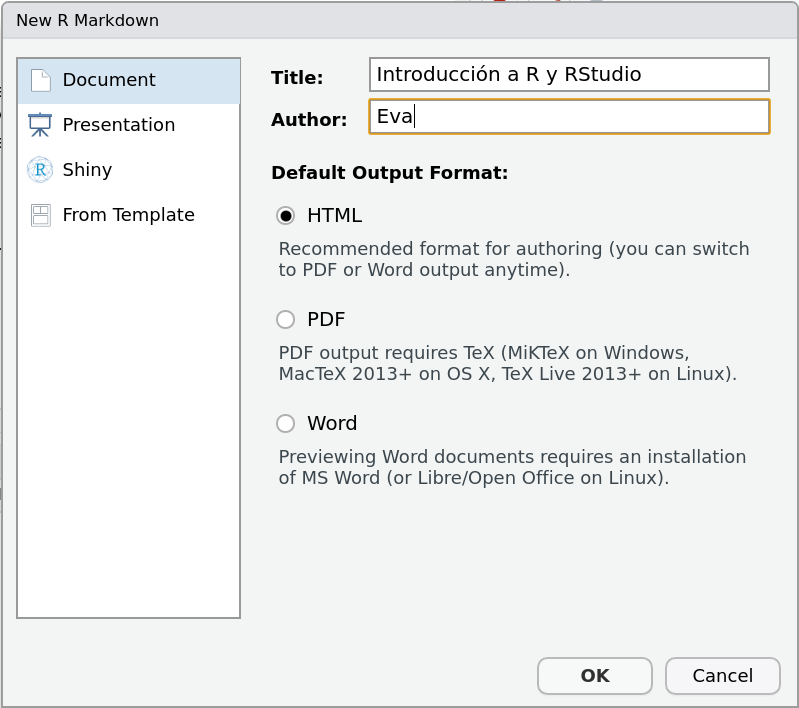
\includegraphics[width=1\linewidth]{images/new-r-markdown} \end{center}

Rellena `Introducción a R y RStudio' en el campo \textbf{Title} y tu nombre en el campo \textbf{Author}. Para el campo \textbf{Default output format}, conserva la elección `HTML' que aparece por defecto.

Al presionar el botón \textbf{OK} se abrirá una nueva pestaña en el panel de \textsf{RStudio} con el nuevo documento R Markdown. Presiona \texttt{Ctrl\ +\ S} para guardarlo, en la carpeta \texttt{IntroR} que creaste antes para la práctica, con el nombre \texttt{intro-r}. Verifica que la etiqueta de la pestaña del documento cambia de \texttt{Untitled1} a \texttt{intro-r.Rmd}.

Las primeras líneas del archivo (1 a 6), delimitadas por tres guiones (\texttt{-\/-\/-})

\begin{Shaded}
\begin{Highlighting}[]
\CommentTok{{-}{-}{-}}
\AnnotationTok{title:}\CommentTok{ "Introducción a R y RStudio"}
\AnnotationTok{author:}\CommentTok{ "Eva"}
\AnnotationTok{date:}\CommentTok{ "19/4/2021"}
\AnnotationTok{output:}\CommentTok{ html\_document}
\CommentTok{{-}{-}{-}}
\end{Highlighting}
\end{Shaded}

conforman la llamada cabecera YAML del documento. Incluye metadatos como el título, el autor y la fecha y el formato de salida del documento que se generará al compilar.

Las líneas siguientes (8 a 10)

\begin{Shaded}
\begin{Highlighting}[]
\InformationTok{\textasciigrave{}\textasciigrave{}\textasciigrave{}\{r setup, include=FALSE\}}
\InformationTok{knitr::opts\_chunk$set(echo = TRUE)}
\InformationTok{\textasciigrave{}\textasciigrave{}\textasciigrave{}}
\end{Highlighting}
\end{Shaded}

las analizaremos con más detalle en la sección \ref{global-options}.

El resto de líneas (12 en adelante), son los contenidos propiamente dichos del documento. Se trata de unos contenidos de muestra, que enseguida reemplazaremos por nuestros contenidos propios. Pero antes de borrar estos contenidos de muestra, compilaremos el documento para ver el resultado inicial.

\hypertarget{compilaciuxf3n}{%
\subsubsection{Compilación}\label{compilaciuxf3n}}

Para compilar el documento presiona el botón \textbf{Knit} en la barra de herramientas de la pestaña del archivo.

\begin{center}
\includegraphics[width=1\linewidth]{images/knit} \end{center}

El documento compilado aparecerá en el panel \textbf{Viewer}, en la ventana de la zona derecha inferior.
Si el documento no se abre en este panel, sino en una ventana emergente, cierra esa ventana y modifica este comportamiento siguiendo los siguientes pasos:

\begin{enumerate}
\def\labelenumi{\arabic{enumi}.}
\tightlist
\item
  Selecciona el menú
\end{enumerate}

\begin{menu}
Tools \textgreater{} Global Options

\end{menu}

\begin{enumerate}
\def\labelenumi{\arabic{enumi}.}
\setcounter{enumi}{1}
\tightlist
\item
  Se abrirá una ventana de nombre \textbf{Options}. Selecciona la sección \textbf{R Markdown} en el menú lateral e indica
\end{enumerate}

\begin{menu}
Show output preview in: Viewer Pane

\end{menu}

como indica la imagen siguiente:

\begin{center}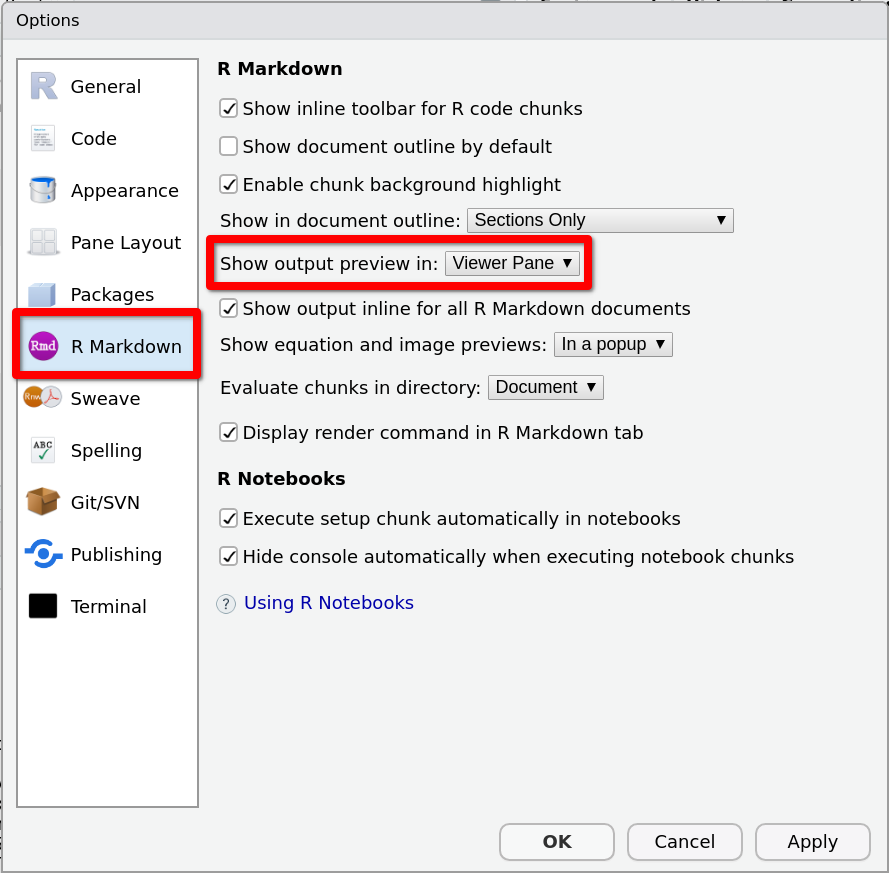
\includegraphics[width=1\linewidth]{images/options-r-markdown} \end{center}

Si miras los contenidos de la carpeta \texttt{IntroR} (puedes hacerlo desde el panel \textbf{Files} de \textsf{RStudio}) verás que, como resultado de la compilación del archivo fuente \texttt{intro-r.Rmd}, se ha creado el archivo de salida \texttt{intro-r.html}. Éste es el archivo que estamos visualizando en el visor de documentos. También podríamos abrirlo en el navegador web, pudiendolo hacer desde el propio visor, presionando el icono resaltado en la siguiente imagen:

\begin{center}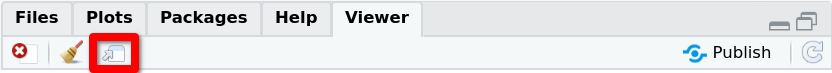
\includegraphics[width=1\linewidth]{images/open-in-new-window} \end{center}

A continuación compararemos el documento fuente \texttt{intro-r.Rmd} con el documento \texttt{intro-r.html} en el visor, para entender cómo se traducen los contenidos que escribimos en un archivo R Markdown en el formato de salida HTML. Nos fíjaremos en particular en los siguientes elementos: encabezados y bloques de código, que se describen en los dos siguientes apartados.

\hypertarget{encabezados}{%
\subsubsection{Encabezados}\label{encabezados}}

Las líneas 12

\begin{Shaded}
\begin{Highlighting}[]
\FunctionTok{\#\# R Markdown }
\end{Highlighting}
\end{Shaded}

y 22

\begin{Shaded}
\begin{Highlighting}[]
\FunctionTok{\#\# Including Plots}
\end{Highlighting}
\end{Shaded}

se traducen en la salida como encabezados de secciones. Si inspeccionas el código del archivo \texttt{intro-r.html} verás que se crean elementos de tipo \texttt{\textless{}h2\textgreater{}}. En general,

\begin{Shaded}
\begin{Highlighting}[]
\FunctionTok{\# Título}
\end{Highlighting}
\end{Shaded}

produce un encabezado de nivel 1,

\begin{Shaded}
\begin{Highlighting}[]
\FunctionTok{\#\# Título}
\end{Highlighting}
\end{Shaded}

un encabezado de nivel 2, y así sucesivamente.

Hay que indicar que es una casualidad la coincidencia del símbolo \texttt{\#} para encabezados en el lenguaje Markdown (independiente de \textsf{R} ) y para comentarios en código \textsf{R}.

\hypertarget{bloques-de-cuxf3digo}{%
\subsubsection{Bloques de código}\label{bloques-de-cuxf3digo}}

Los elementos protagonistas del documento son los bloques de código \textsf{R} (\emph{code chunks}). En el documento de muestra encontramos dos bloques de código: El primero en las líneas 18-20

\begin{Shaded}
\begin{Highlighting}[]
\InformationTok{\textasciigrave{}\textasciigrave{}\textasciigrave{}\{r cars\}}
\InformationTok{summary(cars)}
\InformationTok{\textasciigrave{}\textasciigrave{}\textasciigrave{}}
\end{Highlighting}
\end{Shaded}

y el segundo en las líneas 26-28

\begin{Shaded}
\begin{Highlighting}[]
\InformationTok{\textasciigrave{}\textasciigrave{}\textasciigrave{}\{r pressure, echo=FALSE\}}
\InformationTok{plot(pressure)}
\InformationTok{\textasciigrave{}\textasciigrave{}\textasciigrave{}}
\end{Highlighting}
\end{Shaded}

Si miras el documento compilado, verás que, para el primer bloque se muestra el código y a continuación la salida o resultado de su ejecución; mientras que para el segundo, se muestra solo la salida, y no el código. Esto es debido a la opción \texttt{echo=FALSE}.

Como se indicó al principio de la sección, la sintaxis general para incluir un bloque de código \textsf{R} en un documento R Markdown es la siguiente:

\begin{Shaded}
\begin{Highlighting}[]
\InformationTok{\textasciigrave{}\textasciigrave{}\textasciigrave{}\{r [etiqueta], [lista de opciones]\}}
\InformationTok{\textless{}código R\textgreater{}}
\InformationTok{\textasciigrave{}\textasciigrave{}\textasciigrave{}}
\end{Highlighting}
\end{Shaded}

Las etiquetas de los dos bloques de código del documento de muestra son \texttt{cars} y \texttt{presure}. La etiqueta de un bloque de código sirve para identificarlo, podemos interpretarlo como su nombre, pero es opcional y puede omitirse.

El primer bloque de código no tiene ninguna opción. Y el segundo tiene la opción \texttt{echo=TRUE}, que como acabamos de decir inhibe la impresión del código en el documento compilado.

Puesto que la etiqueta y la lista de opciones son opcionales, el esqueleto básico de un bloque de código \textsf{R} incluido en un documento R Markdown es

\begin{Shaded}
\begin{Highlighting}[]
\InformationTok{\textasciigrave{}\textasciigrave{}\textasciigrave{}\{r\}}
\InformationTok{\textless{}código R\textgreater{}}
\InformationTok{\textasciigrave{}\textasciigrave{}\textasciigrave{}}
\end{Highlighting}
\end{Shaded}

En el cuerpo del bloque podemos escribir instrucciones de \textsf{R} igual que si estuvieramos escribiendo en un script (incluidos comentarios precedidos por el carácter \texttt{\#}).

Notar el cambio de enfoque al escribir en un documento R Markdown respecto a escribir en un script:

\begin{itemize}
\item
  En un script, se espera que escribamos código \textsf{R}, y para escribir texto ordinario hemos de usar comentarios utilizando el carácter \texttt{\#}.
\item
  Por el contrario, en un documento R Markdown, se espera que escribamos texto (con posibilidad de incluir la sintaxis propia del lenguaje Markdown), y para escribir código \textsf{R} hemos de incluirlo en un bloque especial delimitado por la línea \texttt{\textasciigrave{}\textasciigrave{}\textasciigrave{}\{r\}} al comienzo y la línea \texttt{\textasciigrave{}\textasciigrave{}\textasciigrave{}} al final.
\end{itemize}

\hypertarget{plantilla-de-r-markdown}{%
\section{Plantilla de R Markdown}\label{plantilla-de-r-markdown}}

En el capítulo anterior hemos explorado los contenidos de muestra del archivo de R Markdown que hemos creado, y conocemos los dos elementos principales a incluir en este tipo de documentos:

\begin{itemize}
\item
  los \textbf{encabezados}, para estructurar nuestro documento en capítulos, secciones, subsecciones \ldots{}
\item
  y los \textbf{bloques de código}, para incluir instrucciones de \textsf{R}.
\end{itemize}

Ahora vamos a reemplazar los contenidos de muestra por nuestros propios contenidos. Crearemos un primer capítulo con un primer bloque de código, y personalizaremos algunas opciones.

Al final de este capítulo tendremos una plantilla para los documentos R Markdown que usaremos en las prácticas y tareas a lo largo del curso.

Y nuestro documento \texttt{intro-r.Rmd} quedará preparado para practicar el código de \textsf{R} que se presenta en los siguientes capítulos de esta práctica.

\hypertarget{primeros-contenidos}{%
\subsection{Primeros contenidos}\label{primeros-contenidos}}

Borra los contenidos de muestra (línea 12 en adelante) y añade la siguiente línea para crear un primer capítulo (encabezado de nivel 1) de título ``Bloques de código'':

\begin{Shaded}
\begin{Highlighting}[]
\FunctionTok{\# Bloques de código}
\end{Highlighting}
\end{Shaded}

Ahora vamos a crear el primer bloque de código. Para escribir su esqueleto usa el atajo

\begin{center}
\texttt{Ctrl\ +\ Alt\ +\ I}

\end{center}

(\texttt{I} de \emph{Insert}) o, alternativamente, el menú

\begin{menu}
Insert \textgreater{} R

\end{menu}

en la barra de herramientas de la pestaña del documento, que se muestra en la siguiente imagen:

\begin{center}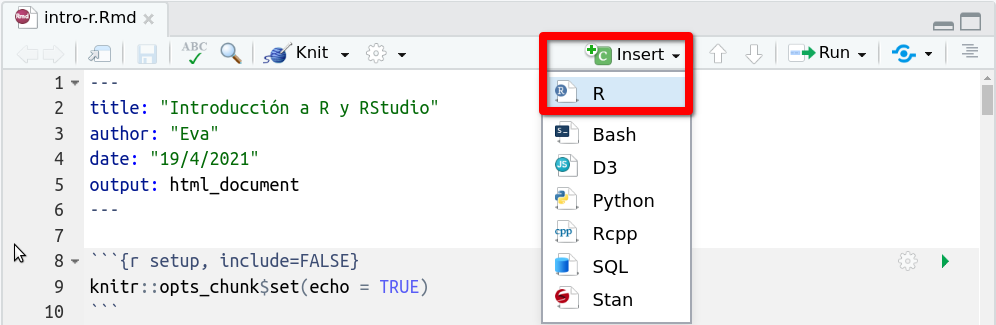
\includegraphics[width=1\linewidth]{images/insert-r} \end{center}

En el bloque de código que acabas de crear añade las instrucciones

\begin{Shaded}
\begin{Highlighting}[]
\NormalTok{sqrt(8)}
\NormalTok{sqrt(10)}
\end{Highlighting}
\end{Shaded}

de forma que los contenidos añadidos queden:

\begin{Shaded}
\begin{Highlighting}[]
\FunctionTok{\# Bloques de código}

\InformationTok{\textasciigrave{}\textasciigrave{}\textasciigrave{}\{r\}}
\InformationTok{sqrt(8)}
\InformationTok{sqrt(10)}
\InformationTok{\textasciigrave{}\textasciigrave{}\textasciigrave{}}
\end{Highlighting}
\end{Shaded}

Compila para ver el resultado.

\hypertarget{algunas-opciones}{%
\subsection{Algunas opciones}\label{algunas-opciones}}

Tras compilar el documento con los contenidos añadidos en la sección anterior, verás que en el documento HTML generado aparecen:

\begin{itemize}
\tightlist
\item
  El código de la primera instrucción \texttt{sqrt(8)}
\item
  Su salida 2.8284271
\item
  El código de la segunda instrucción \texttt{sqrt(10)}
\item
  Su salida 3.1622777
\end{itemize}

Para que se muestre primero el código para las dos instrucciones y a continuación las dos salidas, añade la opción \texttt{results=\textquotesingle{}hold\textquotesingle{}}.

Y para omitir los caracteres \texttt{\#\#} al comienzo de las líneas de la salida, añade la opción \texttt{comment\ =\ \textquotesingle{}\textquotesingle{}}. Nuestro bloque de código con estas dos opciones quedaría:

\begin{Shaded}
\begin{Highlighting}[]
\InformationTok{\textasciigrave{}\textasciigrave{}\textasciigrave{}\{r, results=\textquotesingle{}hold\textquotesingle{}, comment = \textquotesingle{}\textquotesingle{}\}}
\InformationTok{sqrt(8)}
\InformationTok{sqrt(10)}
\InformationTok{\textasciigrave{}\textasciigrave{}\textasciigrave{}}
\end{Highlighting}
\end{Shaded}

Vuelve a compilar y observa el resultado.

\hypertarget{global-options}{%
\subsection{Opciones globales}\label{global-options}}

Al comienzo de nuestro documento, hemos conservado el bloque de código

\begin{Shaded}
\begin{Highlighting}[]
\InformationTok{\textasciigrave{}\textasciigrave{}\textasciigrave{}\{r setup, include=FALSE\}}
\InformationTok{knitr::opts\_chunk$set(echo = TRUE)}
\InformationTok{\textasciigrave{}\textasciigrave{}\textasciigrave{}}
\end{Highlighting}
\end{Shaded}

que estaba incluido en el documento de muestra. Este bloque se identifica con la etiqueta \texttt{setup} y tiene la opción \texttt{include=FALSE}, que hace que, al compilar el documento, si bien se ejecutará la instrucción que contiene, no se incluirá en el formato HTML de salida.

Se explica a continuación el significado de la instrucción \texttt{knitr::opts\_chunk\$set(echo\ =\ TRUE)}: Las opciones especificadas como argumentos de \texttt{knitr::opts\_chunk\$set} (por ahora \texttt{echo=TRUE}) aplicarán a todos los bloques de código que se incluyan en el documento.

Las opciones \texttt{results=\textquotesingle{}hold\textquotesingle{}} y \texttt{comment\ =\ \textquotesingle{}\textquotesingle{}} que hemos aplicado antes a nuestro bloque de código tendrían un efecto local, es decir, aplicarían solo al bloque en el que se han especificado, y si queremos usarlas en los nuevos bloques que creemos, habría que escribirlas de nuevo en todos ellos.

Para aplicar las opciones \texttt{results=\textquotesingle{}hold\textquotesingle{}} y \texttt{comment\ =\ \textquotesingle{}\textquotesingle{}} a todos los bloques de código del documento, las añadiremos como argumentos de \texttt{knitr::opts\_chunk\$set}, de forma que quede:

\begin{Shaded}
\begin{Highlighting}[]
\NormalTok{knitr::opts\_chunk$set(}
\NormalTok{    echo = TRUE,}
\NormalTok{    results=\textquotesingle{}hold\textquotesingle{},}
\NormalTok{    comment = \textquotesingle{}\textquotesingle{}}
\NormalTok{)}
\end{Highlighting}
\end{Shaded}

Ahora, estas dos nuevas opciones aplicarán a todos los bloques, sin necesidad de repetirlas de forma individual en cada uno de ellos, así que puedes borrarlas del bloque de código que creaste antes.

\hypertarget{ejecuciuxf3n-de-instrucciones-individuales}{%
\subsection{Ejecución de instrucciones individuales}\label{ejecuciuxf3n-de-instrucciones-individuales}}

Cuando compilamos un documento R Markdown, se ejecutan todos los bloques de código que contenga, y en el documento compilado podemos visualizar, tanto el código como la salida o resultado (siempre que no hay opciones como \texttt{echo=FALSE} o \texttt{include=FALSE} que inhiban la impresión del código y/o de la salida).

Pero también podemos ejecutar determinadas instrucciones de forma individual, sin necesidad de compilar el documento completo.
Para ello, podemos proceder exactamente igual que en el caso de los scripts, es decir:

\begin{itemize}
\item
  Para ejecutar una sola instrucción, situamos el cursor en cualquiera de las líneas que compongan la instrucción y presionamos \texttt{Ctrl\ +\ Enter}.
\item
  Para ejecutar varias instrucciones, seleccionamos las correspondientes líneas y presionamos \texttt{Ctrl\ +\ Enter}.
\end{itemize}

La salida se mostrará en la consola, y también incrustada en el propio documento, justo debajo del correspondiente bloque de código. Para esto último ha de estar marcada la opción \textbf{Show output inline for all R Markdown documents} en las opciones para R Markdown en el menú

\begin{menu}
Tools \textgreater{} Global options \ldots{} \textgreater{} R Markdown

\end{menu}

como muestra la siguiente imagen:

\begin{center}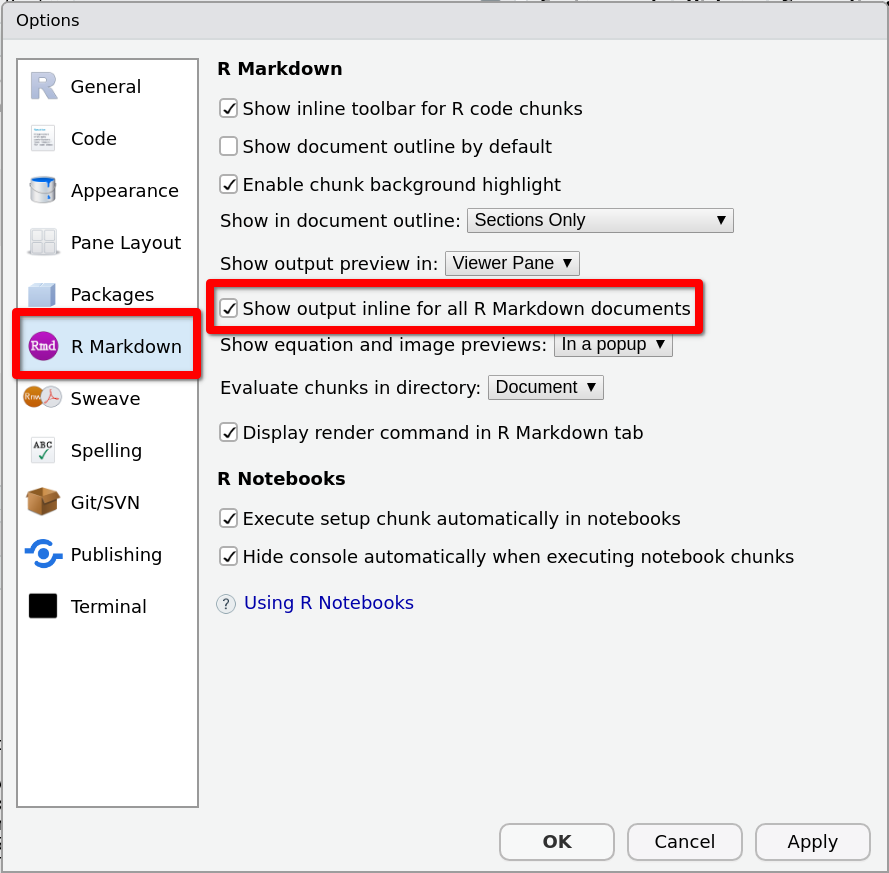
\includegraphics[width=1\linewidth]{images/options-r-markdown-b} \end{center}

Además, podemos ejecutar todas las instrucciones que componen un bloque de código utilizando el botón a la derecha del comienzo del bloque que se resalta en la siguiente imagen:

\begin{center}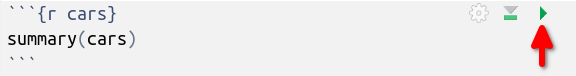
\includegraphics[width=0.8\linewidth]{images/run} \end{center}

\hypertarget{tabla-de-contenidos-flotante}{%
\subsection{Tabla de contenidos flotante}\label{tabla-de-contenidos-flotante}}

Ahora vamos a personalizar el formato de salida para que nuestro documento incluya una tabla de contenidos flotante con las secciones numeradas.

Para ello sustituimos la línea

\begin{Shaded}
\begin{Highlighting}[]
\AnnotationTok{output:}\CommentTok{ html\_document}
\end{Highlighting}
\end{Shaded}

en la cabecera YAML por

\begin{Shaded}
\begin{Highlighting}[]
\AnnotationTok{output:}\CommentTok{ }
\CommentTok{    html\_document:}
\CommentTok{        toc: true}
\CommentTok{        toc\_float: true}
\CommentTok{        number\_sections: true}
\end{Highlighting}
\end{Shaded}

Asegúrate de indentar las líneas conforme se indica, porque el indentado es fundamental para que los campos anidados se lean e interpreten correctamente en el proceso de compilación.

Para que nuestra tabla de contenidos tenga más de una entrada, añade al final del documento un segundo capítulo, con el título de otro capítulo de esta práctica:

\begin{Shaded}
\begin{Highlighting}[]
\FunctionTok{\# Paquetes}
\end{Highlighting}
\end{Shaded}

Compila de nuevo y abre el resultado en el navegador. Verás la tabla de contenidos flotante a la izquierda del cuerpo del documento (o encima del título en pantallas de dimensiones reducidas).

Para apreciar la funcionalidad de la tabla de contenidos flotante, reduce la altura de la ventana del navegador hasta que sea inferior a los contenidos en el cuerpo del documento y aparezca la barra de \emph{scroll} para recorrerlo. Verás que las entradas de la tabla de contenidos actúan como enlaces al inicio de cada capítulo.

\hypertarget{secciones-numeradas}{%
\subsection{Secciones numeradas}\label{secciones-numeradas}}

Para numerar los capítulos añade \texttt{number\_sections:\ true} como opción para el formato de salida:

\begin{Shaded}
\begin{Highlighting}[]
\AnnotationTok{output:}\CommentTok{ }
\CommentTok{    html\_document:}
\CommentTok{        toc: true}
\CommentTok{        toc\_float: true}
\CommentTok{        number\_sections: true}
\end{Highlighting}
\end{Shaded}

\hypertarget{plantilla-final}{%
\subsection{Plantilla final}\label{plantilla-final}}

Después de los cambios que hemos ido haciendo en el documento de muestra, ha debido quedarte así:

\begin{Shaded}
\begin{Highlighting}[]
\CommentTok{{-}{-}{-}}
\AnnotationTok{title:}\CommentTok{ "Introducción a R y RStudio"}
\AnnotationTok{author:}\CommentTok{ "Eva"}
\AnnotationTok{date:}\CommentTok{ "19/4/2021"}
\AnnotationTok{output:}\CommentTok{ }
\CommentTok{    html\_document:}
\CommentTok{        toc: true}
\CommentTok{        toc\_float: true}
\CommentTok{        number\_sections: true}
\CommentTok{{-}{-}{-}}

\InformationTok{\textasciigrave{}\textasciigrave{}\textasciigrave{}\{r setup, include=FALSE\}}
\InformationTok{knitr::opts\_chunk$set(}
\InformationTok{    echo = TRUE,}
\InformationTok{    results=\textquotesingle{}hold\textquotesingle{},}
\InformationTok{    comment = \textquotesingle{}\textquotesingle{}}
\InformationTok{)}
\InformationTok{\textasciigrave{}\textasciigrave{}\textasciigrave{}}

\FunctionTok{\# Bloques de código}

\InformationTok{\textasciigrave{}\textasciigrave{}\textasciigrave{}\{r\}}
\InformationTok{sqrt(8)}
\InformationTok{sqrt(10)}
\InformationTok{\textasciigrave{}\textasciigrave{}\textasciigrave{}}

\FunctionTok{\# Paquetes }
\end{Highlighting}
\end{Shaded}

La primera parte del documento, con la cabecera YAML y el bloque de nombre \texttt{setup} con las opciones de configuración globales para los bloques de código, la repetiremos en todos los documentos R Markdown a lo largo del curso.

\hypertarget{flow}{%
\section{Flujo de trabajo}\label{flow}}

La idea es que, conforme vayas estudiando el resto de la práctica, continúes escribiendo en el documento R Markdown que tienes ahora, después de leer el capítulo anterior.

Así, al terminar de estudiar la práctica, tendrás un informe o resumen de la misma, incluyendo las instrucciones de \textsf{R} que hayas aprendido, los resultados obtenidos, y los comentarios explicativos que hayas añadido.

Incluye bloques de código para practicar el código de \textsf{R} que vayas encontrando en la práctica, así como el texto que creas oportuno para documentar el código que has escrito, de forma que puedas entenderlo cuando releas el documento. En cuanto al seccionado del documento, puedes crear un nuevo capítulo por cada capítulo de la práctica.

Experimenta, escribiendo el código que te apetezca para probar las ideas que te vayan surgiendo y escribiendo el texto que consideres para explicarlas.

Puedes ir compilando cada bloque o instrucción de forma individual, para ver su salida \emph{inline}, y compilar el documento completo cada cierto tiempo.

\hypertarget{packages}{%
\section{Paquetes}\label{packages}}

Cuando instalamos \textsf{R} por primera vez estamos instalando el software \textsf{base R}, que contiene las funciones básicas que se usan regularmente en la mayoría de análisis estadísticos.

Un \textbf{paquete} de R es una colección de funciones, datos y documentación, que extiende las capacidades iniciales de la base de \textsf{R}. Existen multitud de paquetes de \textsf{R}, en su mayoría desarrollados por la comunidad de usuarios de \textsf{R}, que añaden funciones para propósitos específicos.

\href{https://www.tidyverse.org/}{\texttt{tidyverse}} es una colección de paquetes para ciencia de datos que comparten una filosofía común y están diseñados para funcionar juntos de forma natural.
La mayoría de paquetes que usaremos a lo largo del curso forman parte de \texttt{tidyverse}, de forma que instalando este \emph{meta-paquete} tendrás acceso a todos ellos.

\hypertarget{install}{%
\subsection{Instalar un paquete}\label{install}}

Al instalar un paquete descargamos el código que compone dicho paquete en nuestro equipo.
Para instalar un paquete nuevo se utiliza la función \texttt{install.packages()}. La instalación de un paquete se realiza una sola vez, así que la usaremos desde la consola. El paquete \texttt{tidyverse} se instalaría ejecutando la siguiente instrucción:

\begin{Shaded}
\begin{Highlighting}[]
\FunctionTok{install.packages}\NormalTok{(}\StringTok{"tidyverse"}\NormalTok{)}
\end{Highlighting}
\end{Shaded}

La instalación de este paquete puede llevar unos 5-10 minutos, hay que esperar hasta ver en la consola de \textsf{RStudio} que se ha completado el proceso.

\begin{infobox}

\textbf{Nota para Ubuntu:} Si obtienes error al intentar instalar \texttt{tidyverse} en Ubuntu, y el mensaje de la salida contiene la siguiente línea:

\texttt{Package\ libcurl\ was\ not\ found\ in\ the\ pkg-config\ search\ path.}

puedes solucionarlo siguiendo los siguientes pasos:

\begin{enumerate}
\def\labelenumi{\arabic{enumi}.}
\tightlist
\item
  Abre la terminal de Ubuntu y ejecuta
\end{enumerate}

\begin{Shaded}
\begin{Highlighting}[]
\FunctionTok{sudo}\NormalTok{ apt install libcurl4{-}openssl{-}dev libssl{-}dev libxml2{-}dev}
\end{Highlighting}
\end{Shaded}

\begin{enumerate}
\def\labelenumi{\arabic{enumi}.}
\setcounter{enumi}{1}
\tightlist
\item
  En la consola de \textsf{RStudio} vuelve a solicitar la instalación de \texttt{tidyverse} ejecutando
\end{enumerate}

\begin{Shaded}
\begin{Highlighting}[]
\FunctionTok{install.packages}\NormalTok{(}\StringTok{"tidyverse"}\NormalTok{)}
\end{Highlighting}
\end{Shaded}

\end{infobox}

\hypertarget{cargar-un-paquete}{%
\subsection{Cargar un paquete}\label{cargar-un-paquete}}

Para cargar un paquete previamente instalado hay que usar la función \texttt{library()}. Por ejemplo, para cargar el paquete \texttt{tidyverse} escribimos

\begin{Shaded}
\begin{Highlighting}[]
\FunctionTok{library}\NormalTok{(tidyverse)}
\end{Highlighting}
\end{Shaded}

Puedes ignorar los conflictos que se listan en el mensaje que se muestra al cargar \texttt{tidyverse}, no tendrán efectos negativos sobre nuestro código.

Si el paquete está instalado, la instrucción anterior lo cargará y podremos hacer uso de sus funciones.

En caso de no estar instalado, recibiremos un mensaje de error indicando que no existe el paquete solicitado, y habrá que instalarlo primero, como se explicó en el apartado anterior.

Si bien instalación de un paquete (con \texttt{install.packages()}) se realiza una sóla vez, la carga (con \texttt{library()}) es necesaria en cada sesión en la que queramos usar funciones del paquete.

\hypertarget{objects}{%
\section{Objetos en R}\label{objects}}

En este capítulo veremos cómo crear un objeto en \textsf{R} y estudiaremos dos tipos de objetos destacados en \textsf{R}: los \textbf{vectores} y las \textbf{hojas de datos}.

\hypertarget{crear-un-objeto}{%
\subsection{Crear un objeto}\label{crear-un-objeto}}

La instrucción

\begin{Shaded}
\begin{Highlighting}[]
\NormalTok{x }\OtherTok{\textless{}{-}} \DecValTok{2}
\end{Highlighting}
\end{Shaded}

crea una variable u objeto de nombre \texttt{x} y le asigna el valor \(2\).
El operador de asignación en \texttt{R} es \texttt{\textless{}-} (compuesto por el símbolo menor \texttt{\textless{}} y un guión central \texttt{-}).

Puedes comprobar que el objeto \texttt{x} aparece listado en el panel \emph{Environment} de la ventana superior derecha de \textsf{RStudio}. En este panel podemos ver todos los objetos definidos en nuestro entorno o espacio de trabajo (\emph{workspace}).

Cuando se ejecuta una instrucción como la anterior, en la que se asigna un valor u expresión a un objeto, la salida no muestra el valor asignado. Para verlo tenemos que \emph{imprimir} el objeto en cuestión, simplemente escribiendo su nombre:

\begin{Shaded}
\begin{Highlighting}[]
\NormalTok{x }\CommentTok{\# muestra el valor actual de x}
\end{Highlighting}
\end{Shaded}

\begin{Shaded}
\begin{Highlighting}[]
\NormalTok{\#\# [1] 2}
\end{Highlighting}
\end{Shaded}

Una vez definida el objeto o variable \texttt{x} podremos referenciarlo en cálculos posteriores. Por ejemplo, al ejecutar la instrucción

\begin{Shaded}
\begin{Highlighting}[]
\NormalTok{x}\SpecialCharTok{\^{}}\DecValTok{2{-}3}
\end{Highlighting}
\end{Shaded}

\begin{Shaded}
\begin{Highlighting}[]
\NormalTok{\#\# [1] 1}
\end{Highlighting}
\end{Shaded}

obtendremos la salida \(1\) (resultado de \(2^2-3 = 1\)).

\hypertarget{vectores}{%
\subsection{Vectores}\label{vectores}}

Para crear \textbf{vectores} en \textsf{R} usamos la función \texttt{c} (inicial de \emph{concatenate} o \emph{combine}). La instrucción

\begin{Shaded}
\begin{Highlighting}[]
\NormalTok{v }\OtherTok{\textless{}{-}} \FunctionTok{c}\NormalTok{(}\DecValTok{1}\NormalTok{, }\DecValTok{3}\NormalTok{, }\DecValTok{5}\NormalTok{, }\DecValTok{7}\NormalTok{, }\DecValTok{9}\NormalTok{)}
\end{Highlighting}
\end{Shaded}

crea un vector de nombre \texttt{v} formado por los primeros \(5\) números impares. Observa la entrada que se ha creado para \texttt{v} en el panel Environment.

Para acceder al elemento número \texttt{i} del vector \texttt{v} se escribe \texttt{v{[}i{]}} (ojo, que el primer índice es \texttt{1}, no \texttt{0}). Por, ejemplo para extraer el segundo elemento de \texttt{v} escribimos

\begin{Shaded}
\begin{Highlighting}[]
\NormalTok{v[}\DecValTok{2}\NormalTok{]}
\end{Highlighting}
\end{Shaded}

\begin{Shaded}
\begin{Highlighting}[]
\NormalTok{\#\# [1] 3}
\end{Highlighting}
\end{Shaded}

La instrucción

\begin{Shaded}
\begin{Highlighting}[]
\NormalTok{v}\SpecialCharTok{\^{}}\DecValTok{2}
\end{Highlighting}
\end{Shaded}

\begin{Shaded}
\begin{Highlighting}[]
\NormalTok{\#\# [1]  1  9 25 49 81}
\end{Highlighting}
\end{Shaded}

devuelve el vector cuyos elementos son los cuadrados de los elementos de \texttt{v}.
La mayoría de funciones de \textsf{R} que reciben argumentos numéricos aplicadas a un vector numérico operan sobre cada elemento del vector (se dice que están vectorizadas).

\hypertarget{hojas-de-datos}{%
\subsection{Hojas de datos}\label{hojas-de-datos}}

Las hojas de datos (en inglés \emph{data frames}) son la clase de objetos que se usan en \textsf{R} para almacenar los datos obtenidos en un experimento y poder analizarlos.

Empezaremos explorando la hoja de datos de nombre \texttt{mpg} (\textbf{m}iles \textbf{p}er \textbf{g}allon), proporcionada por el paquete \texttt{ggplot2}(que ya hemos cargado al cargar el paquete \texttt{tidyverse}). Esta hoja de datos trata sobre el consumo de combustible de diferentes modelos de coches.

Para cargar la hoja de datos \texttt{mpg} en tu espacio de trabajo escribe

\begin{Shaded}
\begin{Highlighting}[]
\FunctionTok{data}\NormalTok{(}\StringTok{"mpg"}\NormalTok{)}
\end{Highlighting}
\end{Shaded}

Verás que \texttt{mpg} aparece listada en el panel Environment. Inicialmente está catalogada como \texttt{\textless{}Promise\textgreater{}}, pero en cuanto hagamos click en esa celda (o escribamos el nombre de la variable para usarla en nuestro código), se completará la carga y podremos leer que tiene \(234\) observaciones de \(11\) variables. Utilizando los iconos que se resaltan en la imagen siguiente, obtenemos más información sobre la hoja de datos.

\begin{center}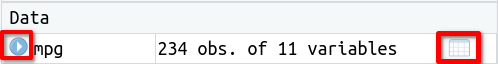
\includegraphics[width=0.6\linewidth]{images/df} \end{center}

\begin{itemize}
\item
  Presionando el icono de la izquierda, vemos los nombres de las 11 variables y sus valores para las primeras observaciones.
\item
  Presionando el icono de la derecha, podremos visualizar la hoja de datos completa. El dato en la celda correspondiente a la fila \(i\) y la columna \(j\) es el valor observado para el coche número \(i\) de la variable número \(j\).
\end{itemize}

En general, una hoja de datos es una especie de matriz u hoja de cálculo, donde las filas representan unidades experimentales, casos u observaciones (en nuestro ejemplo coches) y las columnas representan variables que describen características de interés de las unidades experimentales (en nuestro caso fabricante, modelo, cilindrada, consumo de combustible \ldots). Las celdas contienen los valores observados para cada variable en cada unidad experimental.

Para obtener una descripción de la hoja de datos, escribe \texttt{mpg} en el campo de búsqueda del panel \textbf{Help} de \textsf{RStudio}. También puedes escribir \texttt{?mpg} o \texttt{help(mpg)} en la consola. La página de ayuda explica que la hoja de datos tiene \(234\) filas, donde cada fila representa un coche, y \(11\) variables, que describen diferentes características de los coches. Nos vamos a centrar en las variables \texttt{displ} y \texttt{hwy}, que nos describen como:

\begin{itemize}
\tightlist
\item
  \texttt{displ}: \emph{engine displacemente, in litres} (cilindrada)
\item
  \texttt{hwy}: \emph{higway miles per gallon} (millas recorridas por galón de combustible en conducción por autopista)
\end{itemize}

Para extraer una de las variables de una hoja de datos se utiliza el formato \texttt{\textless{}nombre\ hoja\textgreater{}\$\textless{}nombre\ variable\textgreater{}}. Por ejemplo, para extraer las cilindradas (variable \texttt{displ}) de la hoja de datos \texttt{mpg} utilizamos la instrucción siguiente:

\begin{Shaded}
\begin{Highlighting}[]
\NormalTok{mpg}\SpecialCharTok{$}\NormalTok{displ}
\end{Highlighting}
\end{Shaded}

\begin{Shaded}
\begin{Highlighting}[]
\NormalTok{\#\#   [1] 1.8 1.8 2.0 2.0 2.8 2.8 3.1 1.8 1.8 2.0 2.0 2.8 2.8 3.1 3.1 2.8 3.1 4.2}
\NormalTok{\#\#  [19] 5.3 5.3 5.3 5.7 6.0 5.7 5.7 6.2 6.2 7.0 5.3 5.3 5.7 6.5 2.4 2.4 3.1 3.5}
\NormalTok{\#\#  [37] 3.6 2.4 3.0 3.3 3.3 3.3 3.3 3.3 3.8 3.8 3.8 4.0 3.7 3.7 3.9 3.9 4.7 4.7}
\NormalTok{\#\#  [55] 4.7 5.2 5.2 3.9 4.7 4.7 4.7 5.2 5.7 5.9 4.7 4.7 4.7 4.7 4.7 4.7 5.2 5.2}
\NormalTok{\#\#  [73] 5.7 5.9 4.6 5.4 5.4 4.0 4.0 4.0 4.0 4.6 5.0 4.2 4.2 4.6 4.6 4.6 5.4 5.4}
\NormalTok{\#\#  [91] 3.8 3.8 4.0 4.0 4.6 4.6 4.6 4.6 5.4 1.6 1.6 1.6 1.6 1.6 1.8 1.8 1.8 2.0}
\NormalTok{\#\# [109] 2.4 2.4 2.4 2.4 2.5 2.5 3.3 2.0 2.0 2.0 2.0 2.7 2.7 2.7 3.0 3.7 4.0 4.7}
\NormalTok{\#\# [127] 4.7 4.7 5.7 6.1 4.0 4.2 4.4 4.6 5.4 5.4 5.4 4.0 4.0 4.6 5.0 2.4 2.4 2.5}
\NormalTok{\#\# [145] 2.5 3.5 3.5 3.0 3.0 3.5 3.3 3.3 4.0 5.6 3.1 3.8 3.8 3.8 5.3 2.5 2.5 2.5}
\NormalTok{\#\# [163] 2.5 2.5 2.5 2.2 2.2 2.5 2.5 2.5 2.5 2.5 2.5 2.7 2.7 3.4 3.4 4.0 4.7 2.2}
\NormalTok{\#\# [181] 2.2 2.4 2.4 3.0 3.0 3.5 2.2 2.2 2.4 2.4 3.0 3.0 3.3 1.8 1.8 1.8 1.8 1.8}
\NormalTok{\#\# [199] 4.7 5.7 2.7 2.7 2.7 3.4 3.4 4.0 4.0 2.0 2.0 2.0 2.0 2.8 1.9 2.0 2.0 2.0}
\NormalTok{\#\# [217] 2.0 2.5 2.5 2.8 2.8 1.9 1.9 2.0 2.0 2.5 2.5 1.8 1.8 2.0 2.0 2.8 2.8 3.6}
\end{Highlighting}
\end{Shaded}

que mostrará el vector con las cilindradas de los \(234\) coches.

\hypertarget{plots}{%
\section{Visualización de datos}\label{plots}}

En este capítulo seguimos trabajando con la hoja de datos \texttt{mpg} que presentamos antes.
Nos planteamos en concreto si los coches con motor más grande (mayor \texttt{displ}) tienen mayor consumo de combustible (menor \texttt{hyw}).

Para responder a la pregunta anterior, vamos a realizar un gráfico de puntos para explorar la relación entre las variables \texttt{displ} (cilindrada) y \texttt{hyw} (millas por galón de combustible):

\begin{Shaded}
\begin{Highlighting}[]
\FunctionTok{ggplot}\NormalTok{(}\AttributeTok{data =}\NormalTok{ mpg) }\SpecialCharTok{+} 
    \FunctionTok{geom\_point}\NormalTok{(}\AttributeTok{mapping =} \FunctionTok{aes}\NormalTok{(}\AttributeTok{x =}\NormalTok{ displ, }\AttributeTok{y =}\NormalTok{ hwy)) }
\end{Highlighting}
\end{Shaded}

\begin{center}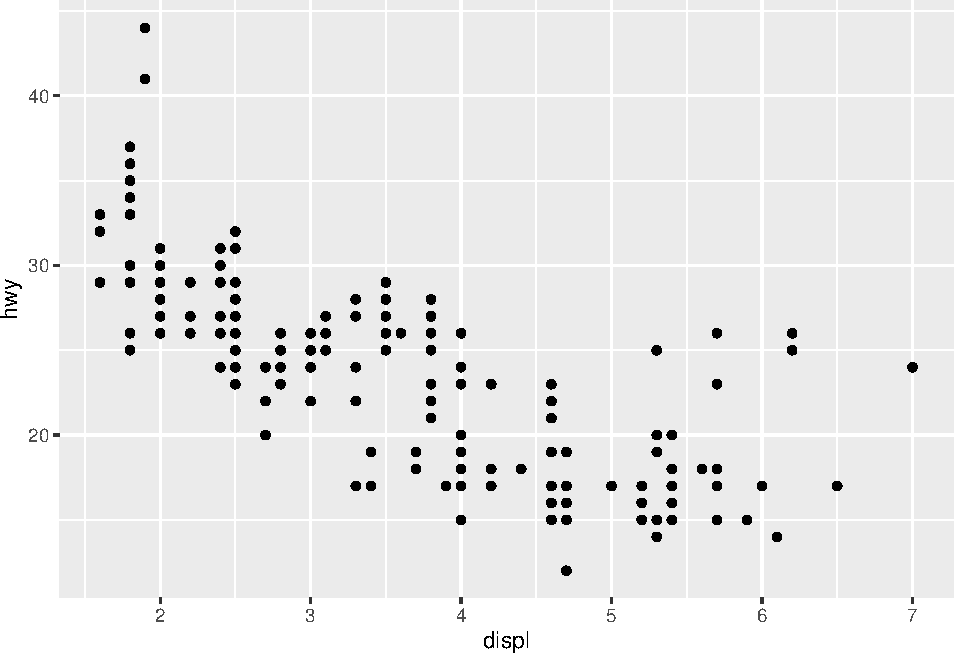
\includegraphics[width=1\linewidth]{basics-R-RStudio_files/figure-latex/unnamed-chunk-24-1} \end{center}

Todos los gráficos se inicializan con la función \texttt{ggplot()}. En el código anterior, la línea

\begin{Shaded}
\begin{Highlighting}[]
\FunctionTok{ggplot}\NormalTok{(}\AttributeTok{data =}\NormalTok{ mpg)}
\end{Highlighting}
\end{Shaded}

simplemente indica que en nuestro gráfico usaremos variables de la hoja de datos \texttt{mpg} y crea un gráfico vacío, al que podemos añadir capas utilizando funciones como \texttt{geom\_point()}, que añadirá una capa de puntos. A lo largo del curso veremos otras funciones como \texttt{geom\_bar()}, \texttt{geom\_hist()} y \texttt{geom\_line()} que añaden capas con otros objetos geométricos (barras, líneas \ldots).

Cada función para añadir un objeto geométrico como \texttt{geom\_point()} necesita un argumento de la forma

\begin{Shaded}
\begin{Highlighting}[]
\NormalTok{mapping }\OtherTok{=} \FunctionTok{aes}\NormalTok{(...)}
\end{Highlighting}
\end{Shaded}

En nuestro ejemplo, ese argumento para la función \texttt{geom\_line()} es

\begin{Shaded}
\begin{Highlighting}[]
\NormalTok{mapping }\OtherTok{=} \FunctionTok{aes}\NormalTok{(}\AttributeTok{x =}\NormalTok{ displ, }\AttributeTok{y =}\NormalTok{ hwy)}
\end{Highlighting}
\end{Shaded}

que especifica que, para cada punto en nuestro gráfico, su coordenada \(x\) vendrá definida por el valor de la variable \texttt{displ}, y su coordenada \(y\) se corresponderá con la variable \texttt{hwy}.

En general, en el argumento de la función \texttt{aes()} se especifica una lista de \textbf{correspondencias} (\emph{mapping}) entre cada \textbf{estética} (\emph{aesthetic}) o propiedad visual de los objetos geométricos a dibujar y las variables de nuestra hoja de datos.

\begin{center}\rule{0.5\linewidth}{0.5pt}\end{center}

Ahora vamos a incluir más información en nuestro gráfico estableciendo una correspondencia entre el color de los puntos (otra propiedad estética) y la variable \texttt{class}, que indica el tipo de coche.

\begin{Shaded}
\begin{Highlighting}[]
\FunctionTok{ggplot}\NormalTok{(}\AttributeTok{data =}\NormalTok{ mpg) }\SpecialCharTok{+} 
    \FunctionTok{geom\_point}\NormalTok{(}\AttributeTok{mapping=}\FunctionTok{aes}\NormalTok{(}\AttributeTok{x =}\NormalTok{ displ, }\AttributeTok{y =}\NormalTok{ hwy, }\AttributeTok{color =}\NormalTok{ class))  }
\end{Highlighting}
\end{Shaded}

\begin{center}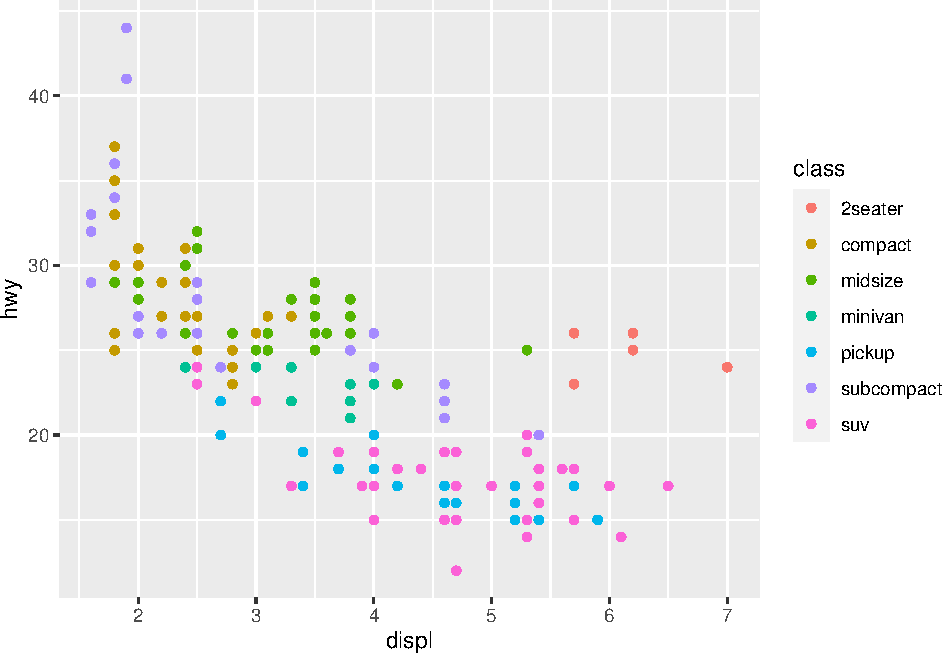
\includegraphics[width=1\linewidth]{basics-R-RStudio_files/figure-latex/unnamed-chunk-28-1} \end{center}

Notar que la inclusión de la correspondencia \texttt{color\ =\ class} ha hecho que \texttt{ggplot2} asigne un color diferente (nivel diferente de la estética \texttt{color}) a cada tipo de coche (valor diferente de la variable \texttt{class}), e incluya una leyenda explicando qué color corresponde a qué tipo de coche.

\begin{center}\rule{0.5\linewidth}{0.5pt}\end{center}

Acabamos personalizando los rótulos de nuestro gráfico con \texttt{labs()}:

\begin{Shaded}
\begin{Highlighting}[]
\FunctionTok{ggplot}\NormalTok{(}\AttributeTok{data =}\NormalTok{ mpg) }\SpecialCharTok{+} 
    \FunctionTok{geom\_point}\NormalTok{(}\AttributeTok{mapping=}\FunctionTok{aes}\NormalTok{(}\AttributeTok{x =}\NormalTok{ displ, }\AttributeTok{y =}\NormalTok{ hwy, }\AttributeTok{color =}\NormalTok{ class)) }\SpecialCharTok{+}
    \FunctionTok{labs}\NormalTok{(}
        \AttributeTok{title =} \StringTok{"Relación entre el tamaño del motor y el consumo de combustible"}\NormalTok{, }
        \AttributeTok{x =} \StringTok{"Cilindrada (litros)"}\NormalTok{,}
        \AttributeTok{y =} \StringTok{"Rendimiento combustible (millas/galón)"}\NormalTok{,}
        \AttributeTok{color =} \StringTok{"Tipo de coche"}
\NormalTok{     )}
\end{Highlighting}
\end{Shaded}

\begin{center}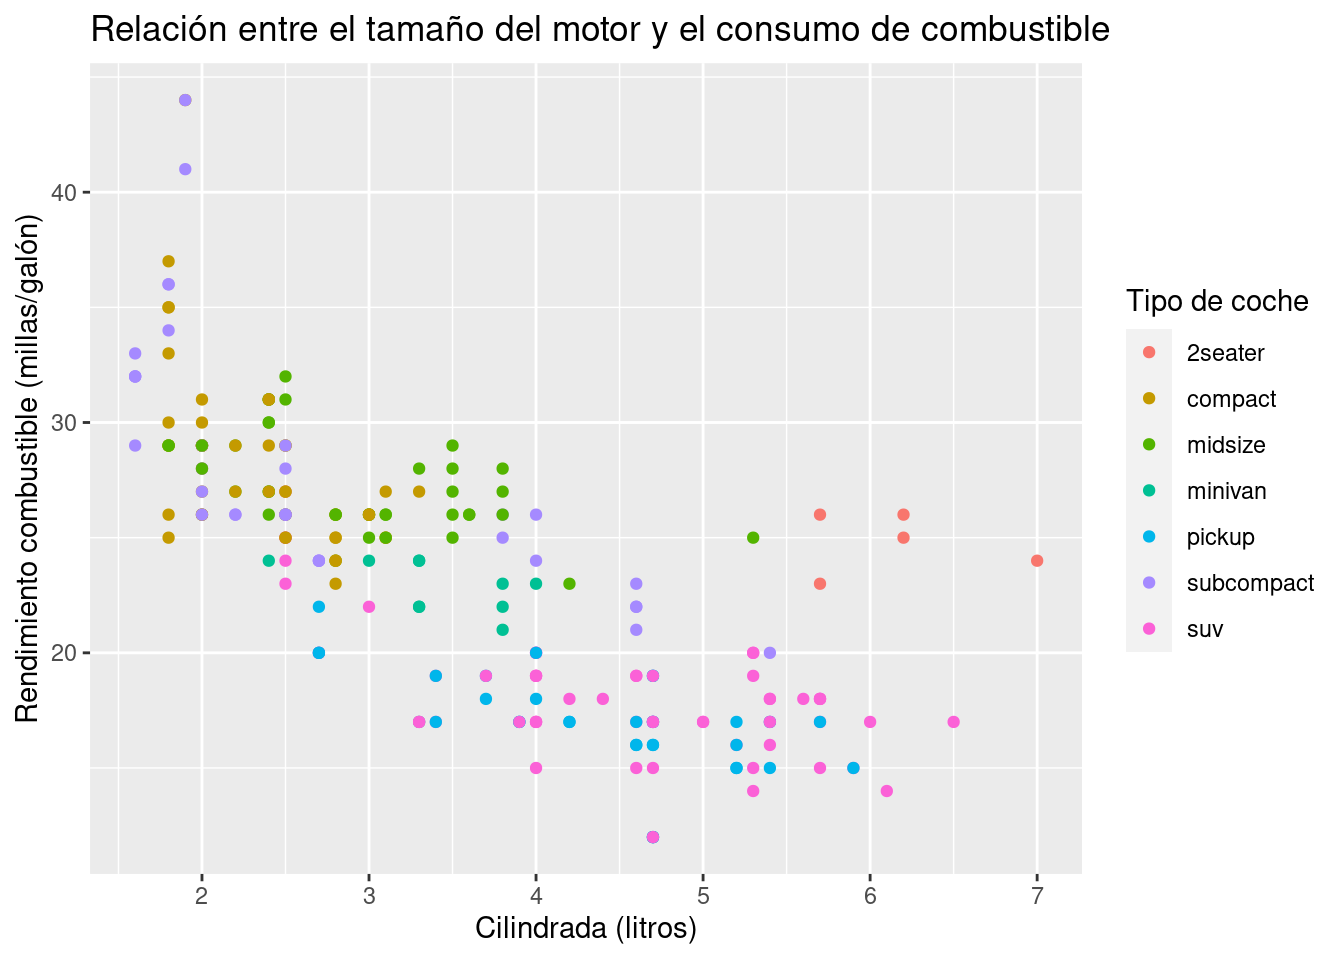
\includegraphics[width=1\linewidth]{basics-R-RStudio_files/figure-latex/unnamed-chunk-29-1} \end{center}

\hypertarget{import}{%
\section{Importar datos}\label{import}}

Hasta ahora hemos trabajado con hojas de datos proporcionadas por paquetes de \textsf{R}, como \texttt{mpg} (de \texttt{ggplot2}). La colección de hojas de datos proporcionada por los diferentes paquetes de \textsf{R} es un buen recurso para enseñar y aprender diferentes tópicos. Pero en la práctica es necesario trabajar con nuestros propios datos o datos extraídos de diversas fuentes.

En este capítulo veremos cómo importar datos en \textsf{R} desde un fichero externo con el paquete \texttt{readr}. El paquete \texttt{readr} forma parte de \texttt{tidyverse} de forma que no es necesario cargarlo individualmente si ya has cargado \texttt{tidyverse}. En concreto, veremos cómo importar los datos contenidos en un archivo CSV (\emph{comma separated values}) con la función \texttt{read\_csv()}.

\hypertarget{los-datos}{%
\subsection{Los datos}\label{los-datos}}

Trabajaremos con un archivo de nombre \texttt{temperaturas.csv}, que contiene las temperaturas máximas y mínimas registradas en el observatorio de la Virgen del Camino para todos los días del mes de abril del año 2018.

Descárgalo pinchando \href{https://drive.google.com/uc?export=download\&id=1xDIvAcQSS4_dFoSIO2hcprhqnbXJqx9r}{aquí} y guárdalo en una carpeta de nombre \texttt{data} en el directorio del archivo R Markdown con el que estés trabajando.

\hypertarget{importar-desde-archivo-local}{%
\subsection{Importar desde archivo local}\label{importar-desde-archivo-local}}

Teniendo el archivo descargado en nuestro equipo, podemos importarlo especificando, como primer argumento de la función \texttt{read\_csv()}, la ruta del archivo, que puede ser local respecto al directorio de trabajo actual.

Con la siguiente instrucción leemos el archivo que hemos descargado y lo almacenamos en un objeto de nombre \texttt{temps}.

\begin{Shaded}
\begin{Highlighting}[]
\NormalTok{temps }\OtherTok{\textless{}{-}} \FunctionTok{read\_csv}\NormalTok{(}\StringTok{"data/temperaturas.csv"}\NormalTok{)}
\end{Highlighting}
\end{Shaded}

Si obtienes algún error indicando que no se encuentra el archivo, puede deberse a que el directorio de trabajo no es el correcto.

\begin{itemize}
\item
  Puedes saber cuál es el directorio de trabajo actual con \texttt{getwd()}.
\item
  Para establecer que el directorio de trabajo sea aquel que contiene a tu archivo R Markdown, selecciona la pestaña de tu archivo .Rmd y utiliza el menú:
\end{itemize}

Session \textgreater{} Set Working Directory \textgreater{} To Source File Location

Si todo ha ido bien, el objeto \texttt{temps} aparecerá en el panel \textbf{Environment} y podrás visualízarlo.

Verás que hay \(30\) filas, una por cada día del mes, y \(3\) columnas con las variables:

\begin{itemize}
\tightlist
\item
  \texttt{Fecha}: fecha del día, en formato año-mes-día
\item
  \texttt{Tmax}: temperatura máxima del día
\item
  \texttt{Tmin}: temperatura mínima del día
\end{itemize}

\hypertarget{importar-desde-url}{%
\subsection{Importar desde URL}\label{importar-desde-url}}

Antes hemos realizado la descarga del archivo de datos de forma manual. También podríamos haberlo hecho desde \textsf{R}, con la función \texttt{download.file()}:

\begin{Shaded}
\begin{Highlighting}[]
\FunctionTok{download.file}\NormalTok{(}
    \AttributeTok{url =} \StringTok{"https://raw.githubusercontent.com/EMazcunan/basics{-}r{-}rstudio/master/data/temperaturas.csv"}\NormalTok{,}
    \AttributeTok{destfile =} \StringTok{"data/temperaturas2.csv"}
\NormalTok{)}
\end{Highlighting}
\end{Shaded}

Comprueba que se ha creado el archivo \texttt{temperaturas2.csv} en la carpeta \texttt{data}.

De hecho, el argumento para especificar el archivo en la función \texttt{read\_csv}, admite una URL. Así que los dos pasos que hemos seguido antes, descargar e importar, pueden hacerse con una sola instrucción:

\begin{Shaded}
\begin{Highlighting}[]
\NormalTok{temps2 }\OtherTok{\textless{}{-}} \FunctionTok{read\_csv}\NormalTok{(}\StringTok{"https://raw.githubusercontent.com/EMazcunan/basics{-}r{-}rstudio/master/data/temperaturas.csv"}\NormalTok{)}
\end{Highlighting}
\end{Shaded}

Después de ejecutar la instrucción anterior, puedes verificar que los objetos \texttt{temps} y \texttt{temps2} son idénticos.

\hypertarget{usar-datos-importados}{%
\subsection{Usar datos importados}\label{usar-datos-importados}}

Una vez que hemos importado los datos de un fichero y los hemos almacenado en un objeto, podemos utilizar dicho objeto como si se tratara de una de las hojas de datos predefinidas en \textsf{R}.

Podemos por ejemplo representar la evolución de las temperaturas mínimas y máximas a lo largo de los días:

\begin{Shaded}
\begin{Highlighting}[]
\FunctionTok{ggplot}\NormalTok{(}\AttributeTok{data =}\NormalTok{ temps) }\SpecialCharTok{+} 
    \FunctionTok{geom\_line}\NormalTok{(}\AttributeTok{mapping =} \FunctionTok{aes}\NormalTok{(}\AttributeTok{x =}\NormalTok{ Fecha, }\AttributeTok{y =}\NormalTok{ Tmin, }\AttributeTok{group  =} \DecValTok{1}\NormalTok{)) }\SpecialCharTok{+} 
    \FunctionTok{geom\_line}\NormalTok{(}\AttributeTok{mapping =} \FunctionTok{aes}\NormalTok{(}\AttributeTok{x =}\NormalTok{ Fecha, }\AttributeTok{y =}\NormalTok{ Tmax, }\AttributeTok{group  =} \DecValTok{1}\NormalTok{)) }
\end{Highlighting}
\end{Shaded}

\begin{center}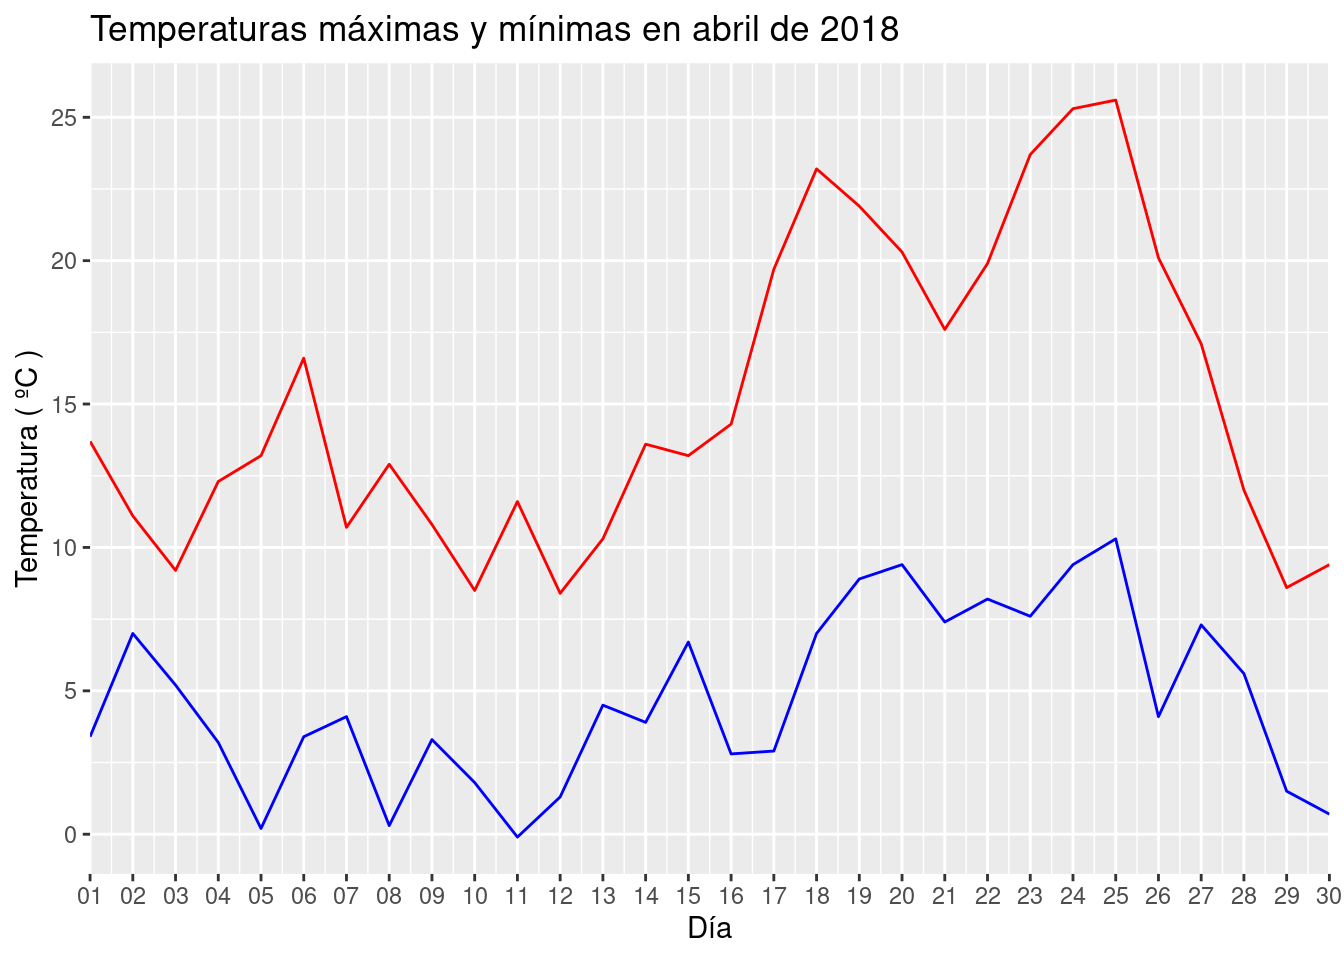
\includegraphics[width=1\linewidth]{basics-R-RStudio_files/figure-latex/unnamed-chunk-33-1} \end{center}

La función \texttt{geom\_line()} actúa primero como si se dibujara un gráfico de puntos con \texttt{geom\_point()} y luego conecta los puntos conforme indique el valor del argumento \texttt{group}. En el caso de nuestros dos diagramas de líneas, queremos que todos los puntos estén conectados, y lo indicamos usando \texttt{group=1}. Cuando hay más variables, la agrupación para las líneas suele hacerse por variable. Si por ejemplo tuvierámos cada día mediciones en varias ciudades, podríamos agrupar para la variable especificando la ciudad.

Cuando varias capas de un gráfico comparten estéticas, esas estéticas comunes pueden especificarse en el argumento de \texttt{ggplot()}. El ejemplo anterior puede acortarse a:

\begin{Shaded}
\begin{Highlighting}[]
\FunctionTok{ggplot}\NormalTok{(}\AttributeTok{data =}\NormalTok{ temps, }\AttributeTok{mapping =} \FunctionTok{aes}\NormalTok{(}\AttributeTok{x =}\NormalTok{ Fecha, }\AttributeTok{group =} \DecValTok{1}\NormalTok{)) }\SpecialCharTok{+} 
    \FunctionTok{geom\_line}\NormalTok{(}\AttributeTok{mapping =} \FunctionTok{aes}\NormalTok{(}\AttributeTok{y =}\NormalTok{ Tmin)) }\SpecialCharTok{+} 
    \FunctionTok{geom\_line}\NormalTok{(}\AttributeTok{mapping =} \FunctionTok{aes}\NormalTok{(}\AttributeTok{y =}\NormalTok{ Tmax)) }
\end{Highlighting}
\end{Shaded}

A continuación tenemos una versión un poco más elaborada del gráfico anterior. Utiliza el paquete \texttt{scales}, que ha de instalarse con \texttt{install.packages("scales")}.

\begin{Shaded}
\begin{Highlighting}[]
\FunctionTok{library}\NormalTok{(scales)}

\FunctionTok{ggplot}\NormalTok{(}\AttributeTok{data =}\NormalTok{ temps, }\FunctionTok{aes}\NormalTok{(}\AttributeTok{x =}\NormalTok{ Fecha, }\AttributeTok{group =} \DecValTok{1}\NormalTok{)) }\SpecialCharTok{+} 
    \FunctionTok{geom\_line}\NormalTok{(}\FunctionTok{aes}\NormalTok{(}\AttributeTok{y =}\NormalTok{ Tmax), }\AttributeTok{color=}\StringTok{"red"}\NormalTok{) }\SpecialCharTok{+} 
    \FunctionTok{geom\_line}\NormalTok{(}\FunctionTok{aes}\NormalTok{(}\AttributeTok{y =}\NormalTok{ Tmin), }\AttributeTok{color=}\StringTok{"blue"}\NormalTok{) }\SpecialCharTok{+} 
    \FunctionTok{scale\_x\_date}\NormalTok{(}
        \AttributeTok{expand =} \FunctionTok{c}\NormalTok{(}\DecValTok{0}\NormalTok{, }\DecValTok{0}\NormalTok{),}
        \AttributeTok{breaks =} \FunctionTok{date\_breaks}\NormalTok{(}\StringTok{"1 day"}\NormalTok{), }
        \AttributeTok{labels =} \FunctionTok{date\_format}\NormalTok{(}\StringTok{"\%d"}\NormalTok{)}
\NormalTok{    ) }\SpecialCharTok{+}
    \FunctionTok{scale\_y\_continuous}\NormalTok{(}\AttributeTok{breaks =} \FunctionTok{seq}\NormalTok{(}\SpecialCharTok{{-}}\DecValTok{5}\NormalTok{, }\DecValTok{30}\NormalTok{, }\DecValTok{5}\NormalTok{)) }\SpecialCharTok{+} 
    \FunctionTok{labs}\NormalTok{(}
        \AttributeTok{title =} \StringTok{"Temperaturas máximas y mínimas en abril de 2018"}\NormalTok{,}
        \AttributeTok{x =} \StringTok{"Día"}\NormalTok{,}
        \AttributeTok{y =} \StringTok{"Temperatura ( ºC )"}
\NormalTok{    )}
\end{Highlighting}
\end{Shaded}

\begin{center}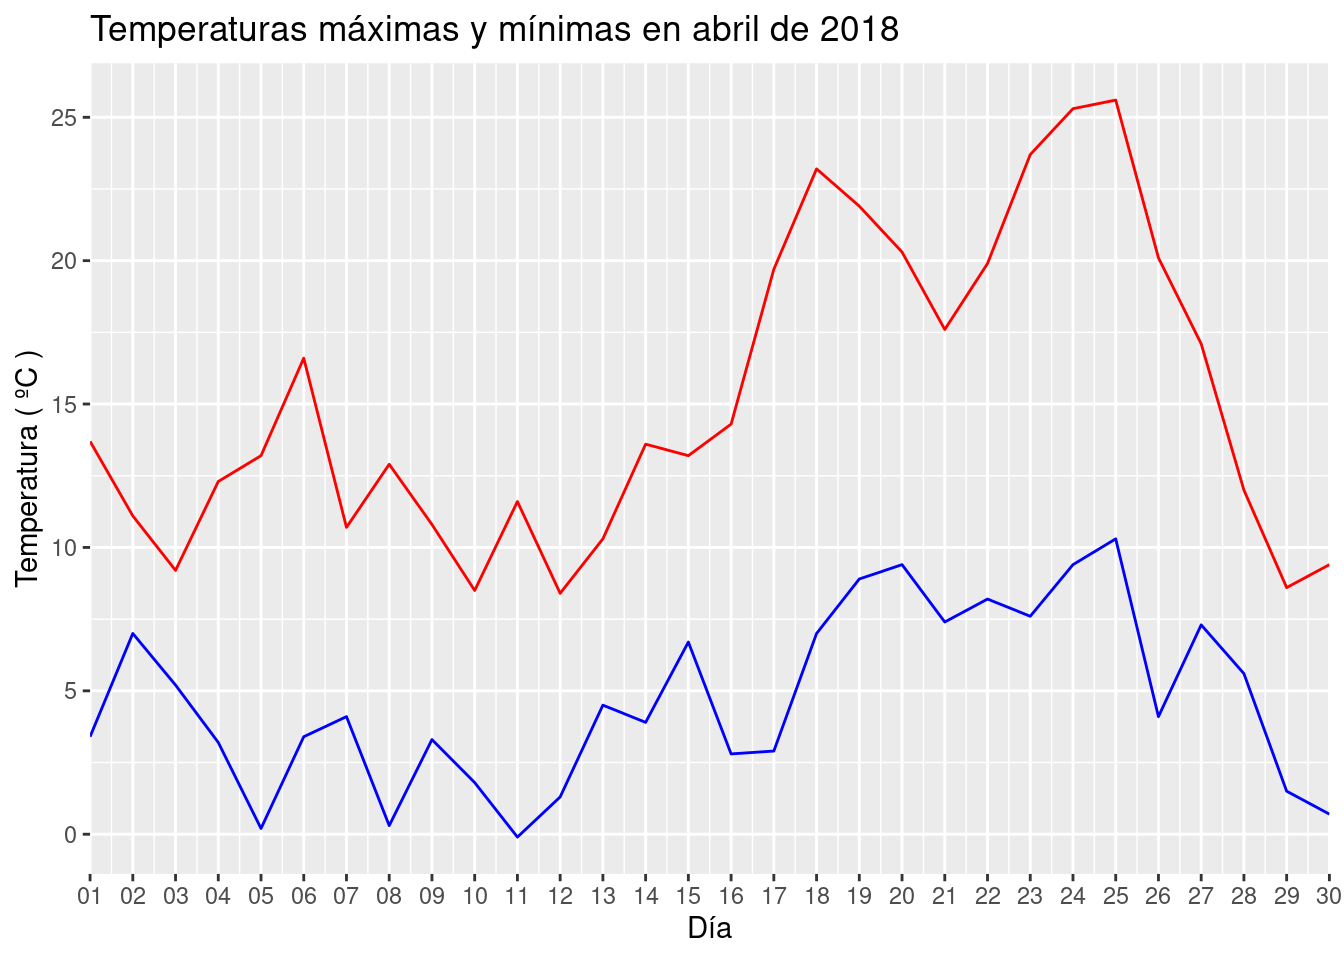
\includegraphics[width=1\linewidth]{basics-R-RStudio_files/figure-latex/unnamed-chunk-35-1} \end{center}

\printbibliography

% This file is created the first time epdf_document is invoked
% but will not be overwriten afterwards.
%
% After Body

\end{document}
